\section[Structuur]{Structuur van Git}
\subsection{Locaties}
\begin{frame}
	3 plekken waar je gegevens zitten:\\
	\vspace{.5cm}
	\begin{tabular}{ll}
		 Working directory			& pas je aan, normale map\\
		 Staging area				& bestanden die je gaat committen\\
		 Repository / \texttt{.git/}&Bevat metadata, objecten
	\end{tabular}
	% edit-stage-commit cyclus
\end{frame}

\subsection{Gegevensstructuur}
\begin{frame}{Wat slaat git op?}
	Geen lijst van wijzigingen, maar kopie\"en (snapshots):
	\begin{center}
		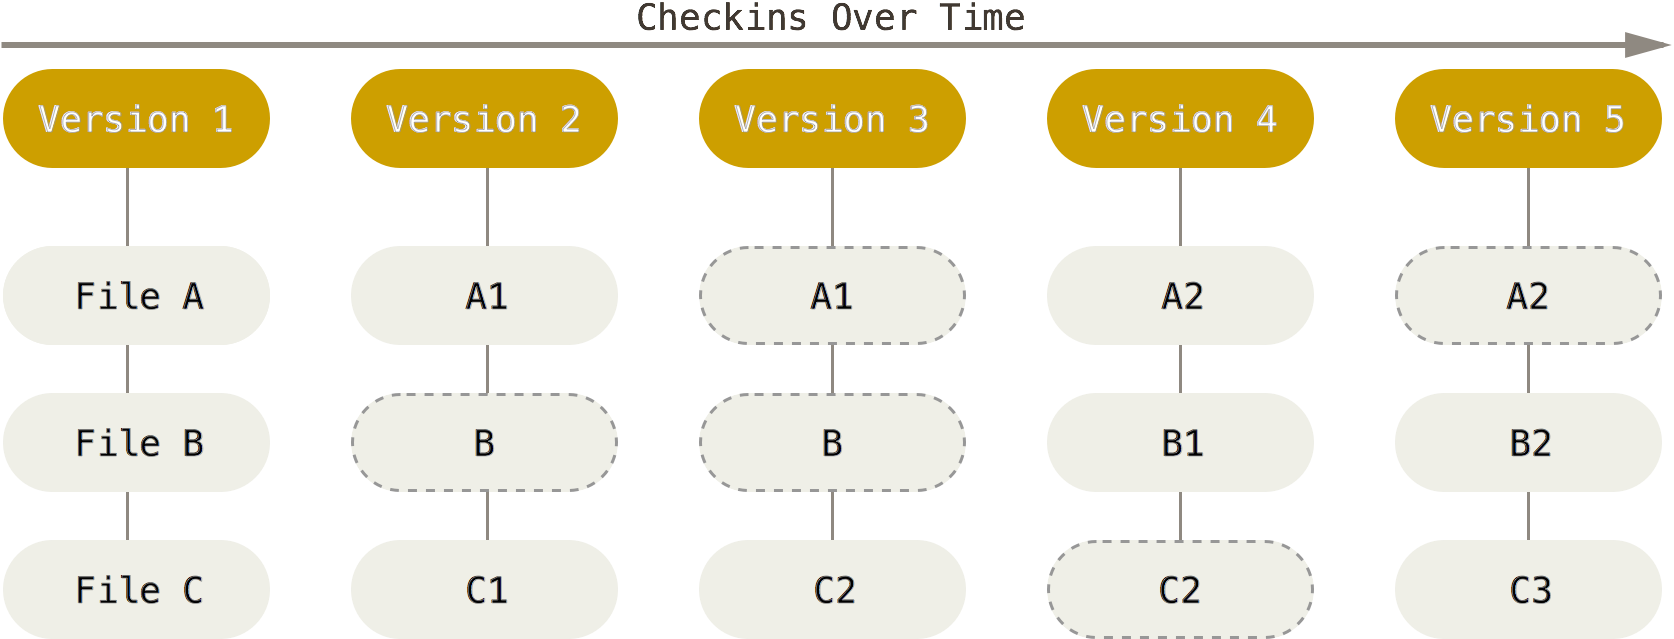
\includegraphics[width=\textwidth]{images/snapshots.png}
	\end{center}
	%(Een version komt hier overeen met een commit, die dus wijst naar versch. versies van bestanden)
\end{frame}

\begin{frame}{Commit}
	\begin{itemize}
		\item Info over jou: (gebruikers)naam + email
		\item Bericht: (hopelijk) korte samenvatting van wat er veranderde
		\item Verwijzing naar set snapshots van bestanden (objects)
		\item Voorganger (merge: 2, initial: 0)
		\item Unieke id (40 tekens)
	\end{itemize}
	\alert{Later (wanneer gedeeld met externe server) niet meer aan (te) passen!}
\end{frame}
